\section{Materiales y Métodos}%
\label{sec:materiales_metodos}

\subsection{Área de estudio}
La cuenca del Plata es una de las diez cuencas fluviales más grandes del mundo, drenando cinco países (parte sur de Brasil, norte de Argentina, Bolivia, Uruguay y Paraguay), representando el $17\%$ de la superficie de América del Sur y sustentando 19 grandes ciudades (con una población superior a $100.000$ habitantes). El río Paraná es el río más grande de esta cuenca, ocupando el noveno lugar entre los ríos más grandes del mundo, según su descarga media anual al océano Atlántico ($18.000 m^{3}/s$;~\cite{LATRUBESSE2008130}). Sin embargo, este río es también uno de los diez principales ríos del mundo en riesgo debido a la presión antropogénica \parencite{wong2007world}.

El estudio se llevó a cabo cerca de la ciudad de Paraná (Argentina), ubicada en la orilla oriental del río, con una población cercana a los $300.000$ habitantes. La recolección, procesamiento y disposición final de los residuos de esta ciudad aún es deficiente, lo que resulta en arroyos urbanos fuertemente contaminados.

Seleccionamos tres áreas de muestreo en los sedimentos de la ribera del río Paraná: aguas arriba de la ciudad (playa Escondida), en la ciudad (playa Thompson, una playa pública municipal) y en una isla ubicada frente a la ciudad (isla Curupí; Fig. \ref{fig:ubicacion_rioParana}), Thompson es una playa recreativa influenciada por la desembocadura de un río urbano fuertemente contaminado (arroyo "Las Viejas") que atraviesa la ciudad de Paraná. Se capturaron peces en las cercanías de los sitios de muestreo. Debido a las condiciones del flujo, esperábamos que el sitio río arriba fuera el menos contaminado, seguido por la isla Curupí, mientras que la playa Thompson, está influenciada por el arroyo "Las Viejas" fuertemente contaminado que cruza la ciudad.

\subsection{Muestreo}
Seleccionamos 2 transectos de $50m$ de largo y $3m$ de ancho para el levantamiento macroplástico (Noik y Tuah, 2015) en cada área de muestreo. Se seleccionaron transectos paralelos a la orilla del río, elegidos al azar, y cubriendo más del $20\%$ de la sección de la costa \parencite{lippiatt2013marine}. Todos los elementos macroplásticos visibles en a superficie de cada transecto se recolectaron a mano.

Los desechos plásticos se clasificaron de acuerdo con el tamaño y se clasificaron como macroplásticos ($>2,5cm$), mesoplásticos ($5mm-2,5cm$) o microplástico ($5mm$). Esta clasificación es utilizada actualmente por el PNUMA \parencite{Cheshire2009}, NOAA \parencite{lippiatt2013marine} y \cite{msfd2013guidance}.

Recolectamos detritos mesoplásticos de muestras por triplicado ($1m^{2}$) ubicadas al azar en cada transecto macroplástico (después de la recolección del macroplástico;~\cite{lippiatt2013marine}). Las partículas de mesoplástico se eliminaron cuidadosamente de los 3 cm superiores de sedimentos de cada cuadrante de $1m^{2}$ (utilizando aceros inoxidables de $5mm$ de tamaño de malla para tamizar los sedimentos). De manera similar, tomamos muestras de microplásticos también por triplicado de los transectos de macroplásticos pero usando cuadrantes más pequeños ($0.25 x 0.25m x 3cm$ de profundidad;~\cite{Klein2015}). Las partículas mesoplásticas se recogieron a mano en el campo utilizando aceros inoxidables (tamaño de malla de $5mm$), mientras que las muestras de microplásticos se transfirieron directamente al laboratorio para su procesamiento.

Todas las muestras (macro y mesoplásticos y sedimentos con microplásticos) se transfirieron al laboratorio para su posterior análisis (ver más abajo).

\begin{figure}[t]
	\centering
	\begin{subfigure}[b]{0.45\linewidth}
		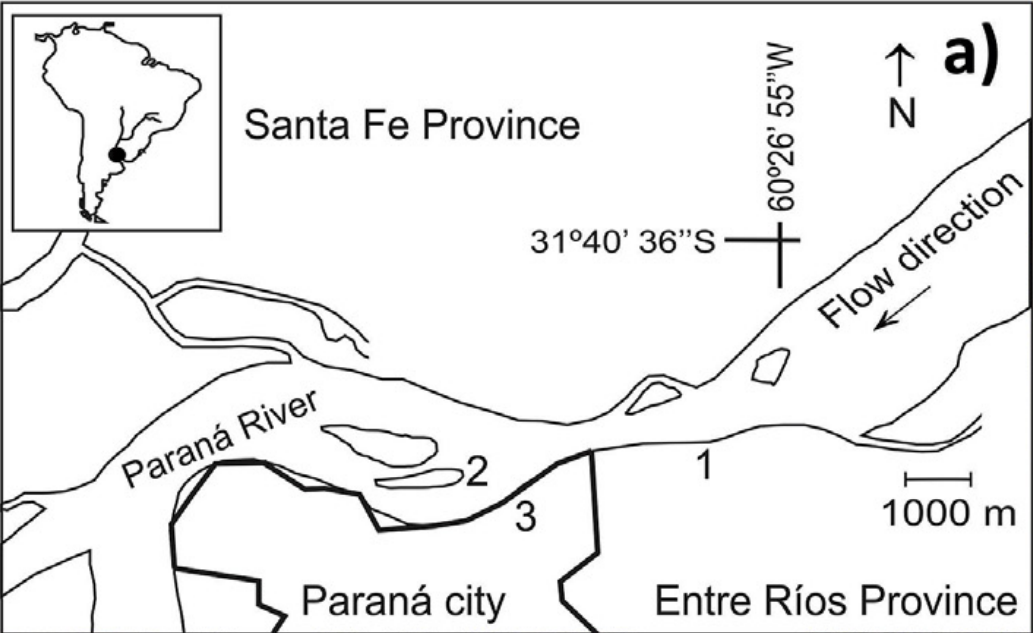
\includegraphics[width=\linewidth]{figura1/figura1a.png}
		\caption{En el Sur Global}
		\label{fig:sur_global}
	\end{subfigure}
	\begin{subfigure}[b]{0.45\linewidth}
		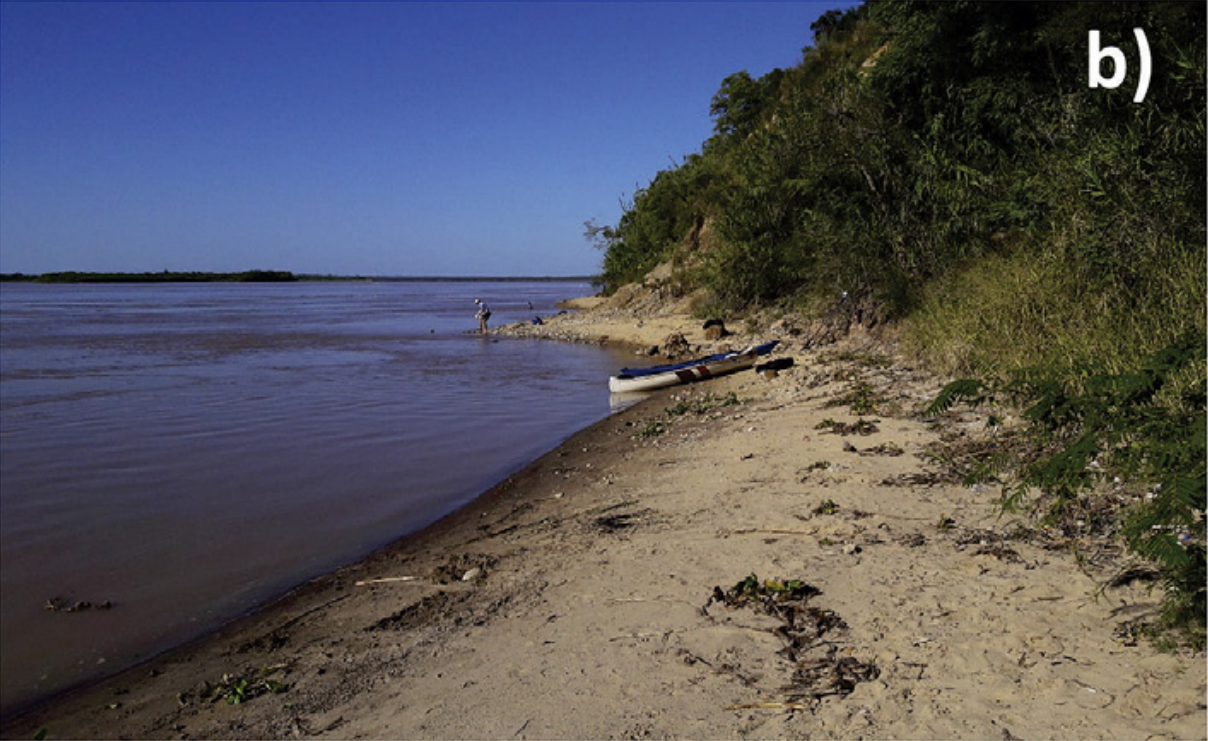
\includegraphics[width=\linewidth]{figura1/figura1b.png}
		\caption{Playa Escondida.}
		\label{fig:playa_escondida}
	\end{subfigure}
	\begin{subfigure}[b]{0.45\linewidth}
		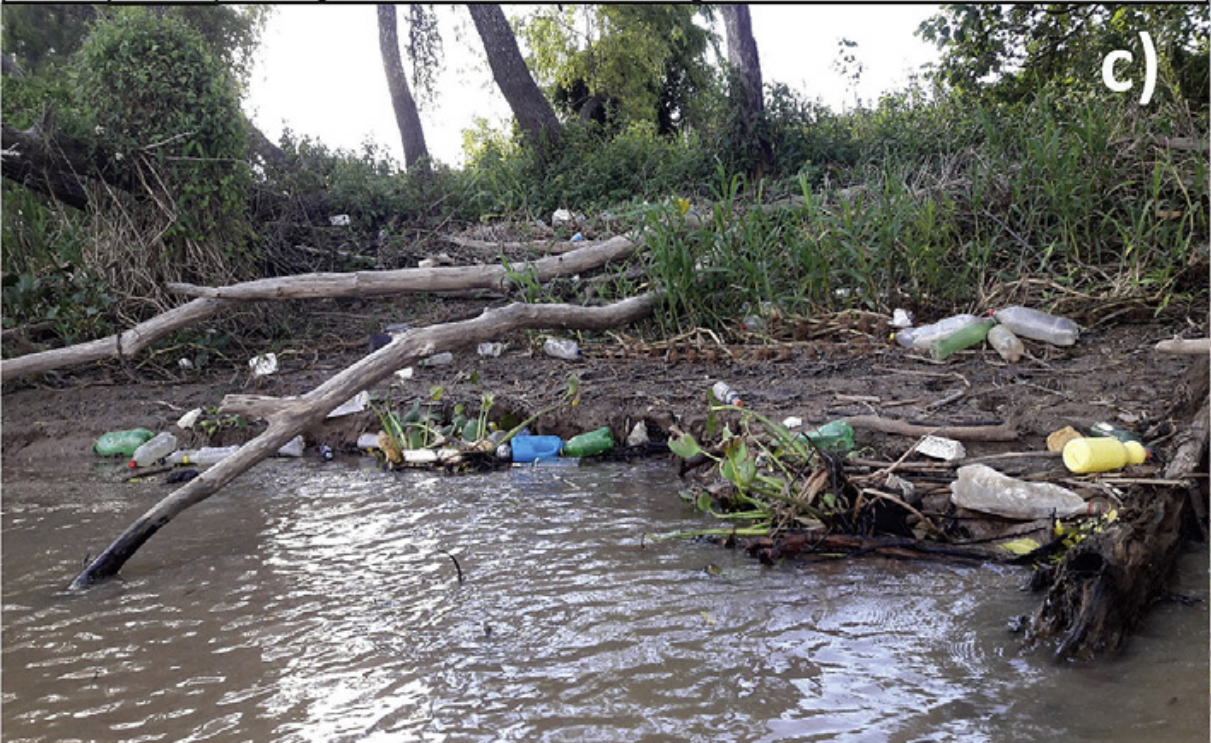
\includegraphics[width=\linewidth]{figura1/figura1c.png}
		\caption{Isla Curupí.}
		\label{fig:isla_curupi}
	\end{subfigure}
	\begin{subfigure}[b]{0.45\linewidth}
		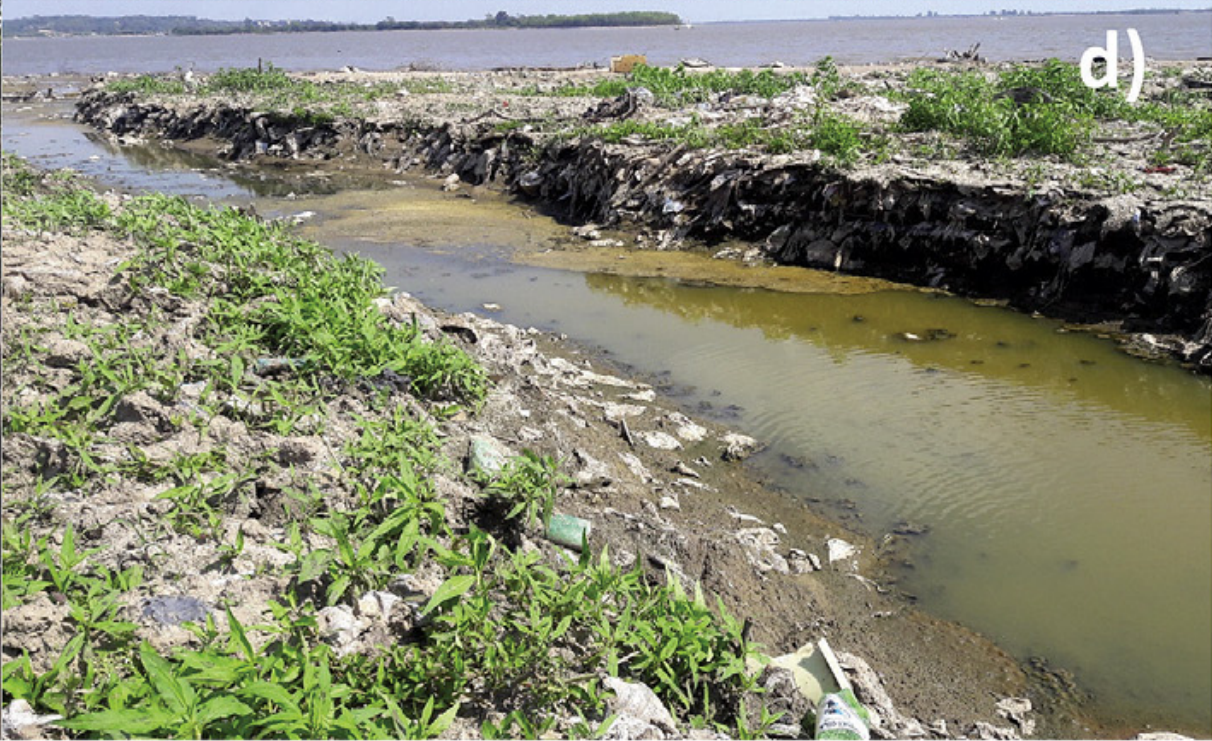
\includegraphics[width=\linewidth]{figura1/figura1d.png}
		\caption{\tiny Playa Thompson (en la confluencia del arroyo urbano Las Viejas con el canal principal de Paraná)}
		\label{fig:playa_thompson}
	\end{subfigure}
	\caption{Ubicación del río Paraná (área de estudio, provincia de Entre Ríos, Argentina)}
	\label{fig:ubicacion_rioParana}
	\vspace{-7mm}
\end{figure}

\textit{Prochilodus lineatus} (localmente llamado ``Sábalo'') es una especie de pez detritívoro dominante de gran importancia para la pesca comercial y artesanal \parencite{espinola2016response}. Para el análisis de peces, se obtuvieron 21 ejemplares frescos que fueron capturados con redes enmalle de $14$ y $16cm$ entre nudos opuestos en los respectivos sitios del área de estudio, respetando las políticas locales. Los peces se capturaron en las primeras horas de la mañana y se transportaron al laboratorio en hielo en 3 horas. Para cada individuo, se midió la longitud total ($cm$) y también se determinó el peso corporal total ($g$). Posteriormente, las muestras de pescado se abrieron con un bisturí y se retiraron los tractos gastrointestinales y se colocaron inmediatamente en cristalería limpia para minimizar el riesgo de contaminación del laboratorio \parencite{BESSA2018575}. Además de los métodos que se describen a continuación, también observamos el color de las partículas ingeridas para identificar las posibles preferencias.

Para evitar la contaminación por microplásticos, potencialmente presentes en el entorno del laboratorio, era obligatorio el uso de batas de laboratorio, guantes y mascarillas de algodón. Además, la cristalería y el lugar de trabajo se limpiaron con una solución de etanol ($96\%$) antes de comenzar todos los experimentos para conservar un ambiente estéril. Desde el inicio de las operaciones hasta la observación al microscopio, las muestras se cubrieron con papel de aluminio.

La materia orgánica presente en las muestras fue digerida con peróxido de hidrógeno ($H_2O_2$)($30\%$) a $60 ^{\circ}C$ (~\cite{PAZOS201785};~\cite{JABEEN2017141}). Según ~\cite{JABEEN2017141}, $H_2O_2$ es un agente oxidante que no cambia ni blanquea la estructura de las partículas microplásticas. De acuerdo con nuestros principios ambientales, todas las campañas de muestreo se realizaron en kayaks (emisión cero y contaminación acústica libre).

\subsection{Análisis y procesamiento de muestras}
Las partículas macroplásticas fueron lavadas, contadas y clasificadas en el laboratorio (ítem por ítem). La clasificación tuvo en cuenta su origen funcional (por ejemplo, envoltorios de alimentos, envases, botellas de bebidas, bolsas de la compra, productos de cuidado personal, etc.) siguiendo la NOAA \parencite{lippiatt2013marine} y la composición de la resina. Se utilizó el Sistema de Codificación de Identificación de Resinas de ASTM Internacional \parencite{RIC} para reconocer la resina plástica utilizada en los macroplásticos manufacturados \parencite{GASPERI2014163}. Como el procedimiento posterior no siempre fue posible de usar (en ocasiones este código se pierde o no es claramente visible), utilizamos un espectrofotómetro FTIR Shimadzu IR Prestige $21^{TM}$ para identificar la resina plástica \parencite{SONG2015202}.

Según ~\cite{GUNDOGDU2017341}, los mesoplásticos se contaron y clasificaron en: espuma de poliestireno, plástico duro, hilo de pescar y películas.

La separación de microplásticos se realizó siguiendo el método propuesto por~\cite{masura2015laboratory}. Por lo tanto, las muestras completas se secaron a $60 ^{\circ}C$ por $24 horas$, se pesaron y se tamizaron a través de un tamiz de acero inoxidable de $350mm$ de tamaño de malla utilizando un agitador de tamices Retsch $^{TM}$. El material restante se transfirió a un vaso de precipitados de $1 L$ para oxidación con peróxido húmedo al $30\%$ ($H_2O_2$) y se colocó en una placa caliente a $60 ^{\circ}C$ hasta que se digerió todo el material orgánico \parencite{T.Yonkos2014}. Una vez completado, se lavó $H_2O_2$ usando agua destilada a través de una malla de $350mm$. Posteriormente, se agregó una solución salina concentrada de $NaCl$ ($1.2 g cm^{-3}$) y se agitó fuertemente durante aproximadamente $1min$ \parencite{Hidalgo-Ruz2012}. Posteriormente, el sobrenadante con microplásticos flotantes se extrajo y se lavó con agua destilada para su posterior procesamiento. Este último paso se repitió tantas veces como fue necesario para atrapar cada partícula de plástico flotante.

Los microplásticos se separaron de otros materiales (presentes en el sobrenadante) y se clasificaron con un microscopio estereoscópico con zoom Boeco$^{tm}$ y un microscopio binocular Nikon$^{TM}$ ($10-40x$). Usamos los criterios sugeridos por~\cite{noren2007small} para identificar microplásticos. Sin embargo, los artículos de origen dudoso se analizaron con un espectrofotómetro FT--IR para confirmar (o rechazar) su composición plástica (~\cite{FRIAS201489};~\cite{LI2016177}). Los rangos de espectros se establecieron en $4000-400 cm^{-1}$, utilizando el software IRsolution Agent. Los espectros resultantes se compararon directamente con las bases de datos de la biblioteca de referencia.

Los microplásticos se clasificaron en espuma de poliestireno (marca registrada de espuma de poliestireno extruido de celda cerrada), plástico duro, película, fibra y rollo de fibra (fibras muy grandes retorcidas), según~\cite{doi:10.1139/cjfas-2014-0281} y ~\cite{GUNDOGDU2017341}.

\subsection{Análisis de datos}
Se crearon tablas y figuras para identificar la presencia, abundancia y tipo de desechos plásticos con el fin de comparar los sitios de muestreo entre sí. Se realizaron correlaciones entre los diferentes rangos de incautación de plástico. Con el fin de probar patrones espaciales de similitud en la abundancia y el tipo de microplásticos, se realizó un análisis canónico de coordenadas principales (CAP). El CAP es un análisis de ordenación restringido que calcula los ejes de coordenadas principales no restringidos seguidos de un análisis discriminante canónico en las coordenadas principales para maximizar la separación entre grupos predefinidos \parencite{anderson2004cap}. El índice de disimilitud de Bray-Curtis y 999 permutaciones fueron los parámetros seleccionados en este procedimiento. Se llevaron a cabo análisis de varianza multivariados permutacionales unidireccionales posteriores (PERMANOVA) \parencite{Anderson2001} para determinar las diferencias entre las puntuaciones del Eje 1 de CAP.

Los análisis estadísticos se realizaron utilizando el software CAP versión 1.0 \parencite{anderson2004cap} y el software MULTIV, versión 2.4.2 \parencite{pillar2006multiv}, con un nivel de significación estadística $p<0.05$.
